\documentclass{article}
\usepackage{graphicx}
\usepackage{amsmath}
\usepackage{amssymb}

% bold vectors
\renewcommand{\vec}[1]{\mathbf{#1}}

% Euclidean vector norm |v|
\newcommand{\norm}[1]{\left\lVert#1\right\rVert}

% matrix transpose v^T
\newcommand{\trans}[1]{#1^\intercal}

% matrix inverse v^-1
\newcommand{\inv}[1]{#1^{-1}}

\title{Dynamic Control of an ROV}
\author{Eric Zheng}

\begin{document}
\maketitle

\section{Introduction}
This document considers the dynamic control of an underwater remotely operated vehicle (ROV). The purpose is to inform Rogue Robotics members in propulsion design decisions for the 2019 MATE ROV competition. This document begins with the basic theoy and then expands into additional dimensions, dynamic considerations, and controller models.

\section{Basic Point Model}
We begin this discussion with an analysis of the basic two-dimensional dynamics of an ideal ROV system (i.e. one not subject to the larger complexities of underwater control). We model the ROV as a rigid body under the influence of $n$ thrusters, each of which are described by a thrust magnitude $f_i$, mounting position $(r_i, \theta_i)$, and mount angle $\psi_i$, as shown in Fig.~\ref{2d}. We are interested in the final output wrench $\vec{F} = \trans{[F_x, F_y, \tau]}$, where $F_x$ is the net force in the $x$-direction, $F_y$ is the net force in the $y$-direction, and $\tau$ is the net torque. More specifically, we are interested in the vector of motor thrusts $\vec{f} = \trans{[f_1, f_2, f_3 \dots f_n]}$ that will produce a desired $\vec{F}$. Note that $\vec{f}$ represents the \emph{influence of the thruster on the ROV}. Newton's first law tells us that this is opposite the direction of the actual thruster exhaust.

\begin{figure}[ht]
  \centering
  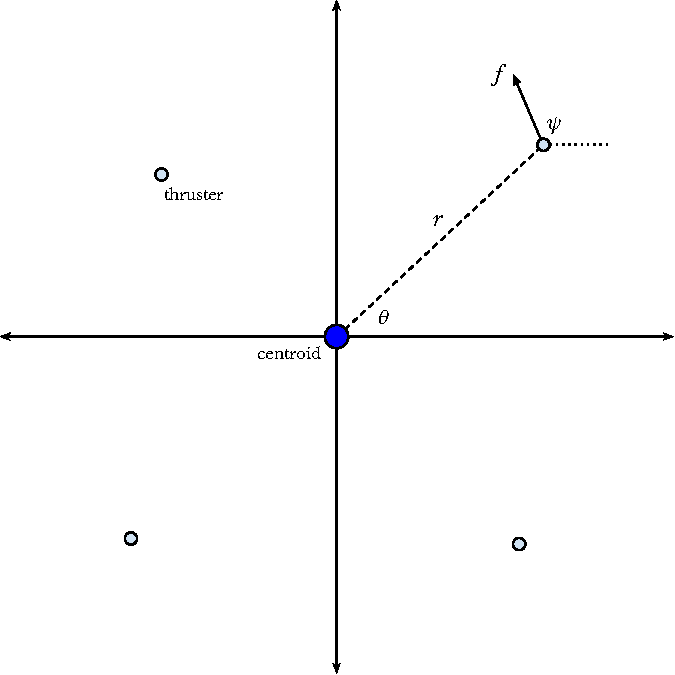
\includegraphics[width=0.75\textwidth]{fig_2d.pdf}
  \caption{Two-dimensional model of the ROV dynamics. The ROV is considered as a rigid body under the influence of $n$ thrusters, each of which exerts a thrust $f$ as shown.}
  \label{2d}
\end{figure}

The mapping $\vec{f} \mapsto \vec{F}$ can be performed with the structure matrix $\vec{A}$, which is defined by the mounting configuration of the thrusters. More specifically, we have:
\begin{equation}
  \vec{F} = \vec{A}\vec{f}
\end{equation}
where:
\begin{equation}
  \vec{A} =
  \begin{bmatrix}
    \cos\psi_1 && \cos\psi_2 && \dots && \cos\psi_n \\
    \sin\psi_1 && \sin\psi_2 && \dots && \sin\psi_n \\
    r_1\sin(\psi_1 - \theta_1) && r_2\sin(\psi_2 - \theta_2) && \dots && r_n\sin(\psi_n - \theta_n)
  \end{bmatrix}
\end{equation}

For $n > 3$, this is an under-determined linear system, which, barring singularities, has infinitely many solutions. (Singularities should be avoidable with a good thruster layout.) We want to choose the \emph{optimal} input vector $\vec{f}$ to achieve our desired output $\vec{F}$; here, we arbitrarily define the optimal solution as the one that minimizes the Euclidean norm $\norm{\vec{f}}$. (Another objective function of interest is the total current draw, but this requires modeling current and thrust.) This optimization problem is easily solvable with numerical methods, which are available, for example, through \verb|scipy|.

Now, let's extend this model to the three-dimensional case. Here, each motor still exerts some thrust $f_i$, but its position is described by the spherical coordinates $(r_i, \theta_i, \phi_i)$, and its thrust orientation is described by a polar angle $\psi_i$ and an azimuthal angle $\alpha_i$. This can be more simply thought of as each thruster being situated at coordinates $(r_i, \theta_i, \phi_i)$ in an ROV-fixed reference frame with the origin at the ROV's centroid. A force described by $(f_i, \psi_i, \alpha_i)$ is then applied in a translated reference frame whose origin is fixed at the thruster, as shown in Fig.~\ref{3d}. We can then similarly model the net forces and torques $\vec{F} = \trans{[F_x, F_y, F_z, \tau_x, \tau_y, \tau_z]}$ on the ROV in terms of the structure matrix $\vec{B}$ and actuation vector $\vec{f}$:
\begin{equation}
  \vec{F} = \vec{B}\vec{f}
\end{equation}
where, for $i$ between $1$ and $n$:
\begin{equation}
  \vec{B} =
  \begin{bmatrix}
    \sin\psi_i\cos\alpha_i \\
    \sin\psi_i\sin\alpha_i \\
    \cos\psi_i \\
    r_i\cos\psi_i\cos\theta_i - r_i\sin\psi_i\cos\alpha_i\sin\theta_i\sin\phi_i \\
    r_i\sin\psi_i\cos\alpha_i\sin\theta_i\cos\phi_i - r_i\cos\psi_i\cos\theta_i \\
    -r_i\sin\psi_i\sin\theta_i\cos(\alpha_i+\phi_i)
  \end{bmatrix}
\end{equation}

To recap, the control problem for the ROV can be stated as this: given a desired net force/torque $\vec{F}$ on the ROV (typically from the joystick input), calculate the motor thrusts $\vec{f}$ needed to produce this desired resultant. In the case of the Rogue Robotics ROV, we have $n=6$, meaning that this is a well-determined system (the matrix $\vec{B}$ is square). Then, in most cases, there is a unique solution vector $\vec{f} = \inv{\vec{B}}\vec{F}$. Since $\vec{B}$ is fixed by the ROV design, We can pre-compute its inverse, making the calculation very fast.

\begin{figure}[ht]
  \centering
  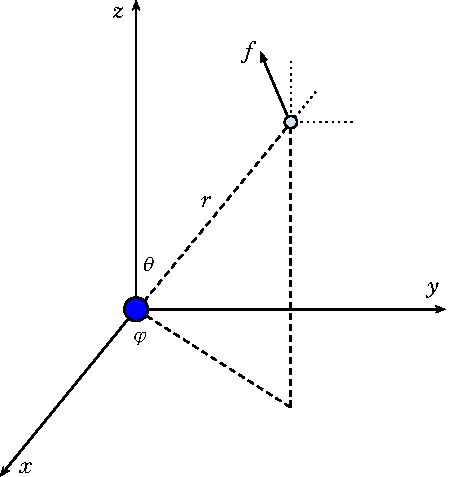
\includegraphics[width=0.75\textwidth]{fig_3d.pdf}
  \caption{Three-dimensional model of ROV dynamics.}
  \label{3d}
\end{figure}

\section{Nonlinear Dynamic Considerations}
This simple dynamic model of the ROV is sufficient for basic joystick control, but more advanced software control needs to take into account the difficulties of navigating underwater. In the submarine environment, the ROV is subject to numerous nonlinear effects, such as added mass and drag forces. These are very difficult to computationally solve, but they can be reasonably estimated from physical data.

I'll get around to proper citations later, but in general, the equations of motion for an ROV can be written as:
\begin{equation}
  \vec{M}\dot{\vec{v}} + C(\vec{v})\vec{v} + D(\vec{v})\vec{v} + g(\vec{\eta}) = \vec{F}
\end{equation}
where $\vec{\eta}$ describes the ROV's position and orientation in a world-fixed reference frame, $\vec{v}$ describes the ROV's linear and angular velocity in a body-fixed reference frame, $\vec{M}$ is the inertia and added mass matrix, $C(\vec{v})$ is the matrix of Coriolis and centripetal effects, $D(\vec{v})$ is the drag force matrix, $g(\vec{\eta})$ is the restoring buoyant and gravitational force matrix, and $\vec{F}$ is the thruster force matrix, described in the preceding section. Note that besides the usual rigid-body inertial terms in the matrix $\vec{M}$, there is also an effective added mass from movement in water.
\end{document}
